
Le tenseur des contraintes $\vec{\vec{\sigma}}$ s'exprime ainsi :
%
\begin{equation}
\vec{\vec{\sigma}} = - p \vec{\vec{I}} + \vec{\vec{\tau}}
\end{equation}
%
avec $\vec{\vec{I}}$ la matrice identité et $\vec{\vec{\tau}}$ le tenseur des contraintes visqueuses.

L'injection de cette définition dans la conservation de la QDM \eqref{eq:QDM} nous donne :
%
\begin{equation}
\rho \frac{D\vec{U}}{Dt} = - \vec{\nabla} p + \vec{\nabla} \cdot \vec{\vec{\tau}} + \rho \vec{f}
\end{equation}

En statique (fluide sans mouvement), on a $\vec{\vec{\tau}} = 0$ et $\vec{U} = \vec{0}$, cette équation nous donne alors le Principe Fondamental de la Statique \eqref{eq:PFS}.

%-------------------------------------------------------
\paragraph{Loi newtonienne :}Elle est valable pour un fluide newtonien (voir partie \ref{sec:rheo} sur la rhéologie).
%
\begin{equation}
\vec{\vec{\tau}} = - \lambda \vec{\nabla} \cdot \vec{U} \vec{\vec{I}} + 2\mu \vec{\vec{D}}
\end{equation}
%
$\vec{\vec{D}}$ est le tenseur des vitesses de déformation (en s\up{-1}), il traduit la déformation des particules fluides avec le mouvement, on calcule ses termes ainsi :
%
\begin{equation}
D_{ij} = \frac{1}{2} \left( \frac{\partial{U_i}}{\partial{x_j}} + \frac{\partial{U_j}}{\partial{x_i}} \right)
\end{equation}

$\mu$ est la viscosité dynamique vur en partie \ref{sec:rheo} et $\lambda$ est le coefficient de seconde viscosité. Dans un cas incompressible, le fait que $\vec{\nabla} \cdot \vec{U} = 0$ implique que $\vec{\vec{\tau}} = 2 \mu \vec{\vec{D}}$. Dans un cas non visqueux on a simplement $\vec{\vec{\tau}} = 0$ (c'est un modèle très simplifié bien sûr).

La viscosité cinématique d'un fluide newtonien s'exprime en m/s\up{2} et est définit ainsi :
%
\begin{equation}
\nu = \frac{\mu}{\rho}
\end{equation}

%-------------------------------------------------------
\paragraph{Théorème de Navier Stokes :}il est simplement composé des équations de conservation de la masse \eqref{eq:masse} et de la QDM \eqref{eq:QDM} dans le cas d'un fluide newtonien, incompressible et homogène. On note qu'on a alors $\vec{\nabla} \cdot \vec{\vec{\tau}} = 2 \mu \vec{\nabla} \cdot \vec{\vec{D}} = \mu \nabla^2 \vec{U}$.
%
\begin{align}[left=\empheqlbrace]
 & \frac{D\vec{U}}{Dt} = - \frac{1}{\rho} \vec{\nabla} p + \nu  \nabla^2 \vec{U} + \vec{f} \\
 \notag & \vec{\nabla} \cdot \vec{U} = 0
\label{eq:navierstokes}
\end{align}


%-------------------------------------------------------
\paragraph{Théorème de Bernouilli :}ses conditions d'application sont les suivantes :

\begin{itemize}
    \item fluide non visqueux
    $\Leftrightarrow \vec{\vec{\sigma}}=-p\vec{\vec{I}}$
    \item écoulement stationnaire
    $\Leftrightarrow \partial{}/\partial{t} = 0$
    \item écoulement incompressible
    $\Leftrightarrow \vec{\nabla} \cdot \vec{U} = 0$
    \item forces massiques dérivant d'un potentiel
    $\Leftrightarrow\vec{f} = - \vec{\nabla} \psi$ (pour la pesenteur $\vec{f} = \vec{g}$ et $\psi = g z$)
\end{itemize}
%
Alors la quantité suivante est constante le long d'une ligne de courant :
%
\begin{equation}
K = p + \frac{1}{2}\rho U^2 + \rho\psi
\label{eq:bernouilli}
\end{equation}

\paragraph{Équations d'Euler :}elles correspondent au théorème de Navier Stokes dans le cas d'un fluide non visqueux ($\nu=0$)

\textbf{Conditions d'adhérence aux limites :}
\begin{itemize}
    \item paroi solide : $\vec{U}_{paroi}=$vitesse de la paroi
    \item interface fluides : $\vec{U}_A=\vec{U}_B$
\end{itemize}

\begin{center}
    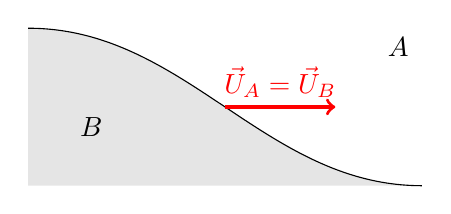
\begin{tikzpicture}
        \fill[color=gray!20] (0,0) -- (0,2) ..controls +(2,0) and +(-2,0).. (5,0) -- (0,0);
        \draw (0,2) ..controls +(2,0) and +(-2,0).. (5,0);
        \draw (0.8,0.5) node[above] {$B$};
        \draw (4.7,2) node[below] {$A$};
        \draw [->,red,very thick] (2.5,1) -- +(1.4,0);
        \draw [red] (3.2,1) node[above] {$\vec{U}_A = \vec{U}_B$};
    \end{tikzpicture}
\end{center}
